\documentclass[aspectratio=169]{beamer}
\usepackage[utf8]{inputenc}
\usepackage{amssymb,amsmath,amsfonts}
\usepackage{natbib}
%\usepackage{showframe}
\usetheme{Pittsburgh}
\usecolortheme{whale}

\setbeamertemplate{footline}[frame number]
\setbeamertemplate{navigation symbols}{}
\bibliographystyle{plain}

\title{Finding Criminal Groups in Suspect Networks Using a Steiner Tree Approach}
\author[]{\textbf{Fredy Troncoso\inst{a}} \and Richard Weber\inst{b} \and Alex Barrales-Araneda\inst{a}}
\institute[]
{\footnotesize
  \inst{a}{Departamento de Ingeniería Industrial,
    Universidad del Bío-Bío}
						
  \inst{b}{Departamento de Ingeniería Industrial,
    Universidad de Chile}
}
\date[]{\footnotesize \vfill 32nd EURO Conference \\ July 6th, 2022. Espoo, Finland}

\begin{document}

\begin{frame}
  \titlepage
\end{frame}

\begin{frame}
  \frametitle{Outline}
  \tableofcontents
\end{frame}

\section[Introduction]{Introduction}

\begin{frame}
\frametitle{Introduction}
  \begin{columns}
  \column{0.5\textwidth}
    \begin{enumerate}
      \item A criminal group is defined as a structured group formed by two or more people that is characterized by serious criminal activity over time, with high internal cohesion and a hierarchical and specialized structure\cite{Hagan06}
      \item The structure of a criminal group is given by the relationships between its members and is fundamental for the success of its operations.\cite{boscaasi}
    \end{enumerate}
  \column{0.5\textwidth}
    \centering
    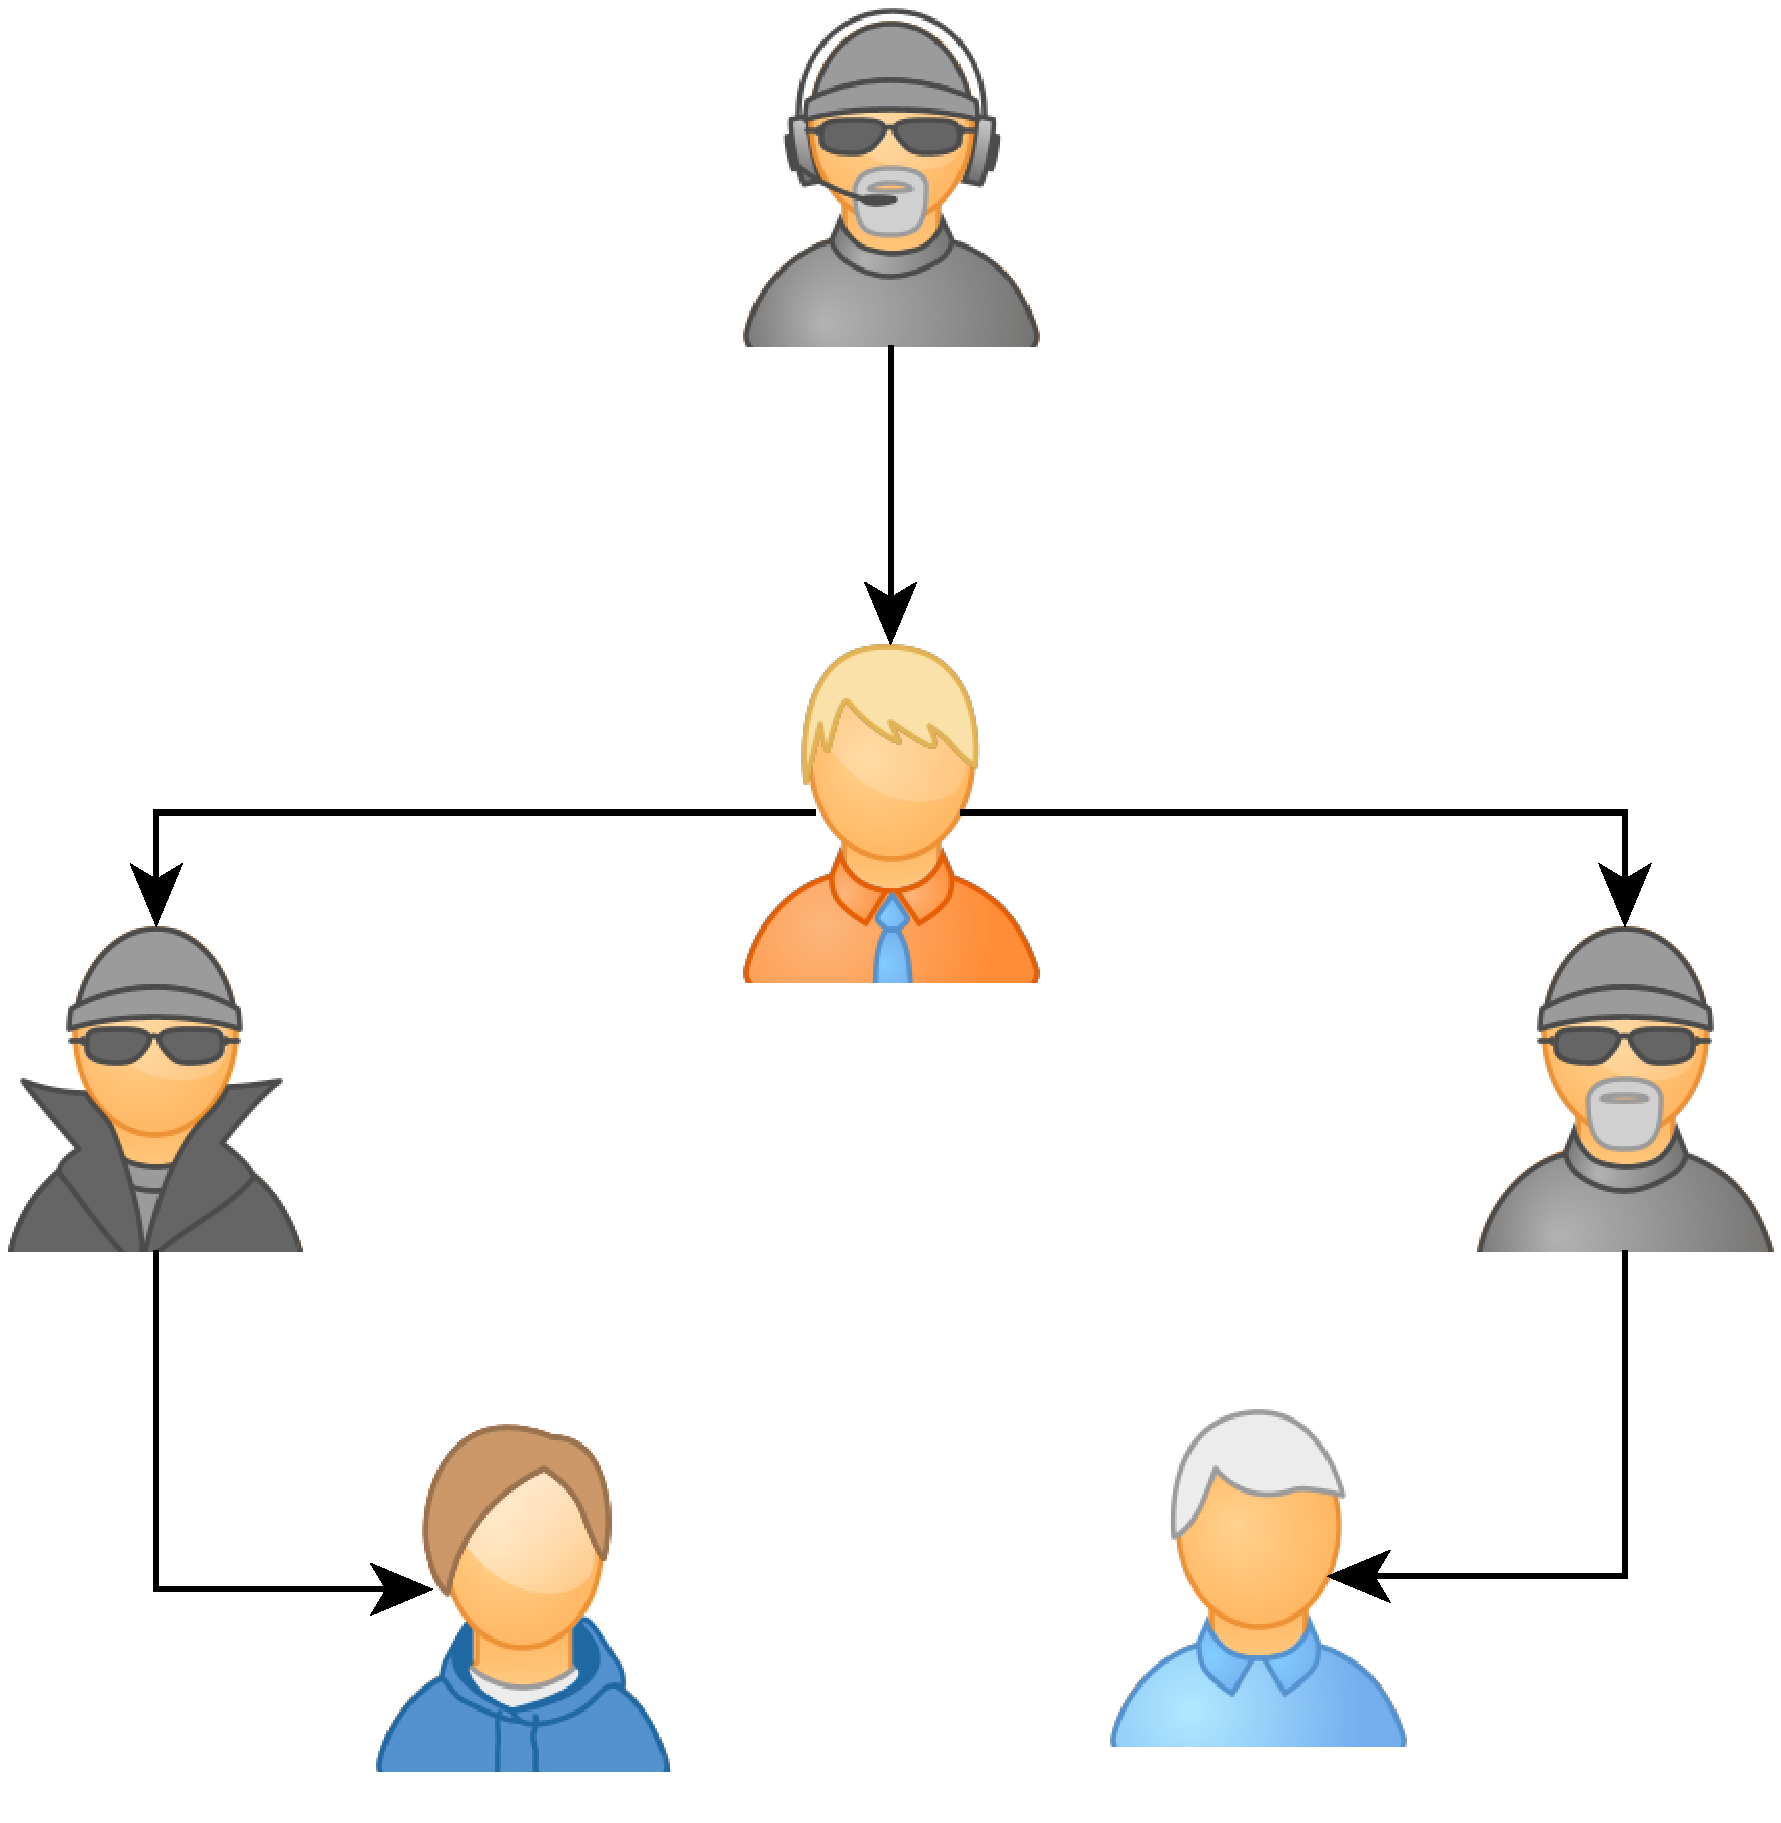
\includegraphics[width=0.9\textwidth]{images/CG.pdf}
  \end{columns}
\end{frame}



\section[Background]{Background}
\subsection[STP]{Node-Weighted Steiner Tree problem}

\begin{frame}
\frametitle{Node-Weighted Steiner Tree problem}
  \begin{columns}
  \column{0.65\textwidth}
    \begin{enumerate}
      \item The STP in graphs is a combinatorial optimization problem that has been widely used in network design, integrated circuit design, localization problems, machine learning, systems biology, and bioinformatics\cite{ljubic2021solving}.
      \item The STP seeks a tree that interconnects a set of nodes $S$ called terminals at a minimum cost.
    \end{enumerate}
  \column{0.35\textwidth}
    \begin{figure}[ht]
      \centering
      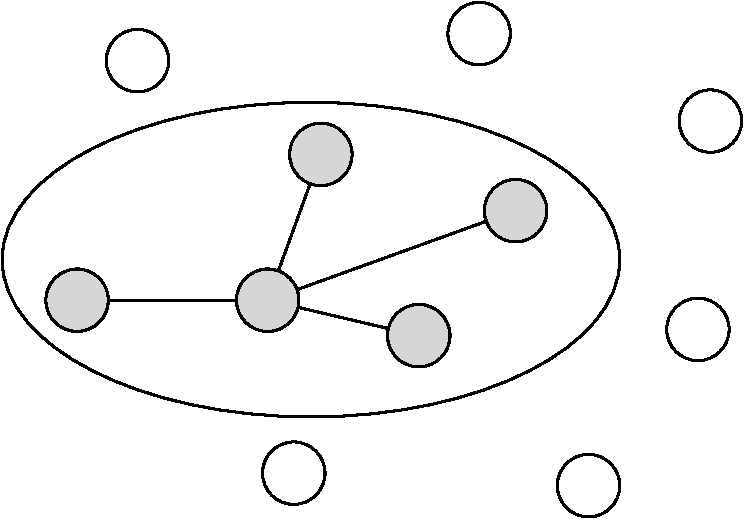
\includegraphics[width=0.9\textwidth]{images/STP.pdf}
      \caption{\footnotesize Figure ? $|S| = 4$}
    \end{figure}
  \end{columns}
\end{frame}

\section[A new model based on Steiner trees]{A new model based on Steiner trees}
\subsection[StRAM]{Steiner tree rational association model}

\begin{frame}
\frametitle{Steiner tree rational association model (StRAM)}
  \begin{columns}
  \column{0.5\textwidth}
    \begin{enumerate}
      \item<1-> The search for association can be seen as the process by which a criminal planner $s$ plans a group crime by choosing other criminals.
      \item<2-> The planner is rational and chooses criminals with the criminal skills that guarantee that the crime is carried out with the maximum utility.
    \end{enumerate}
  \column{0.5\textwidth}
    \begin{figure}[ht]
      \centering
      \only<1> {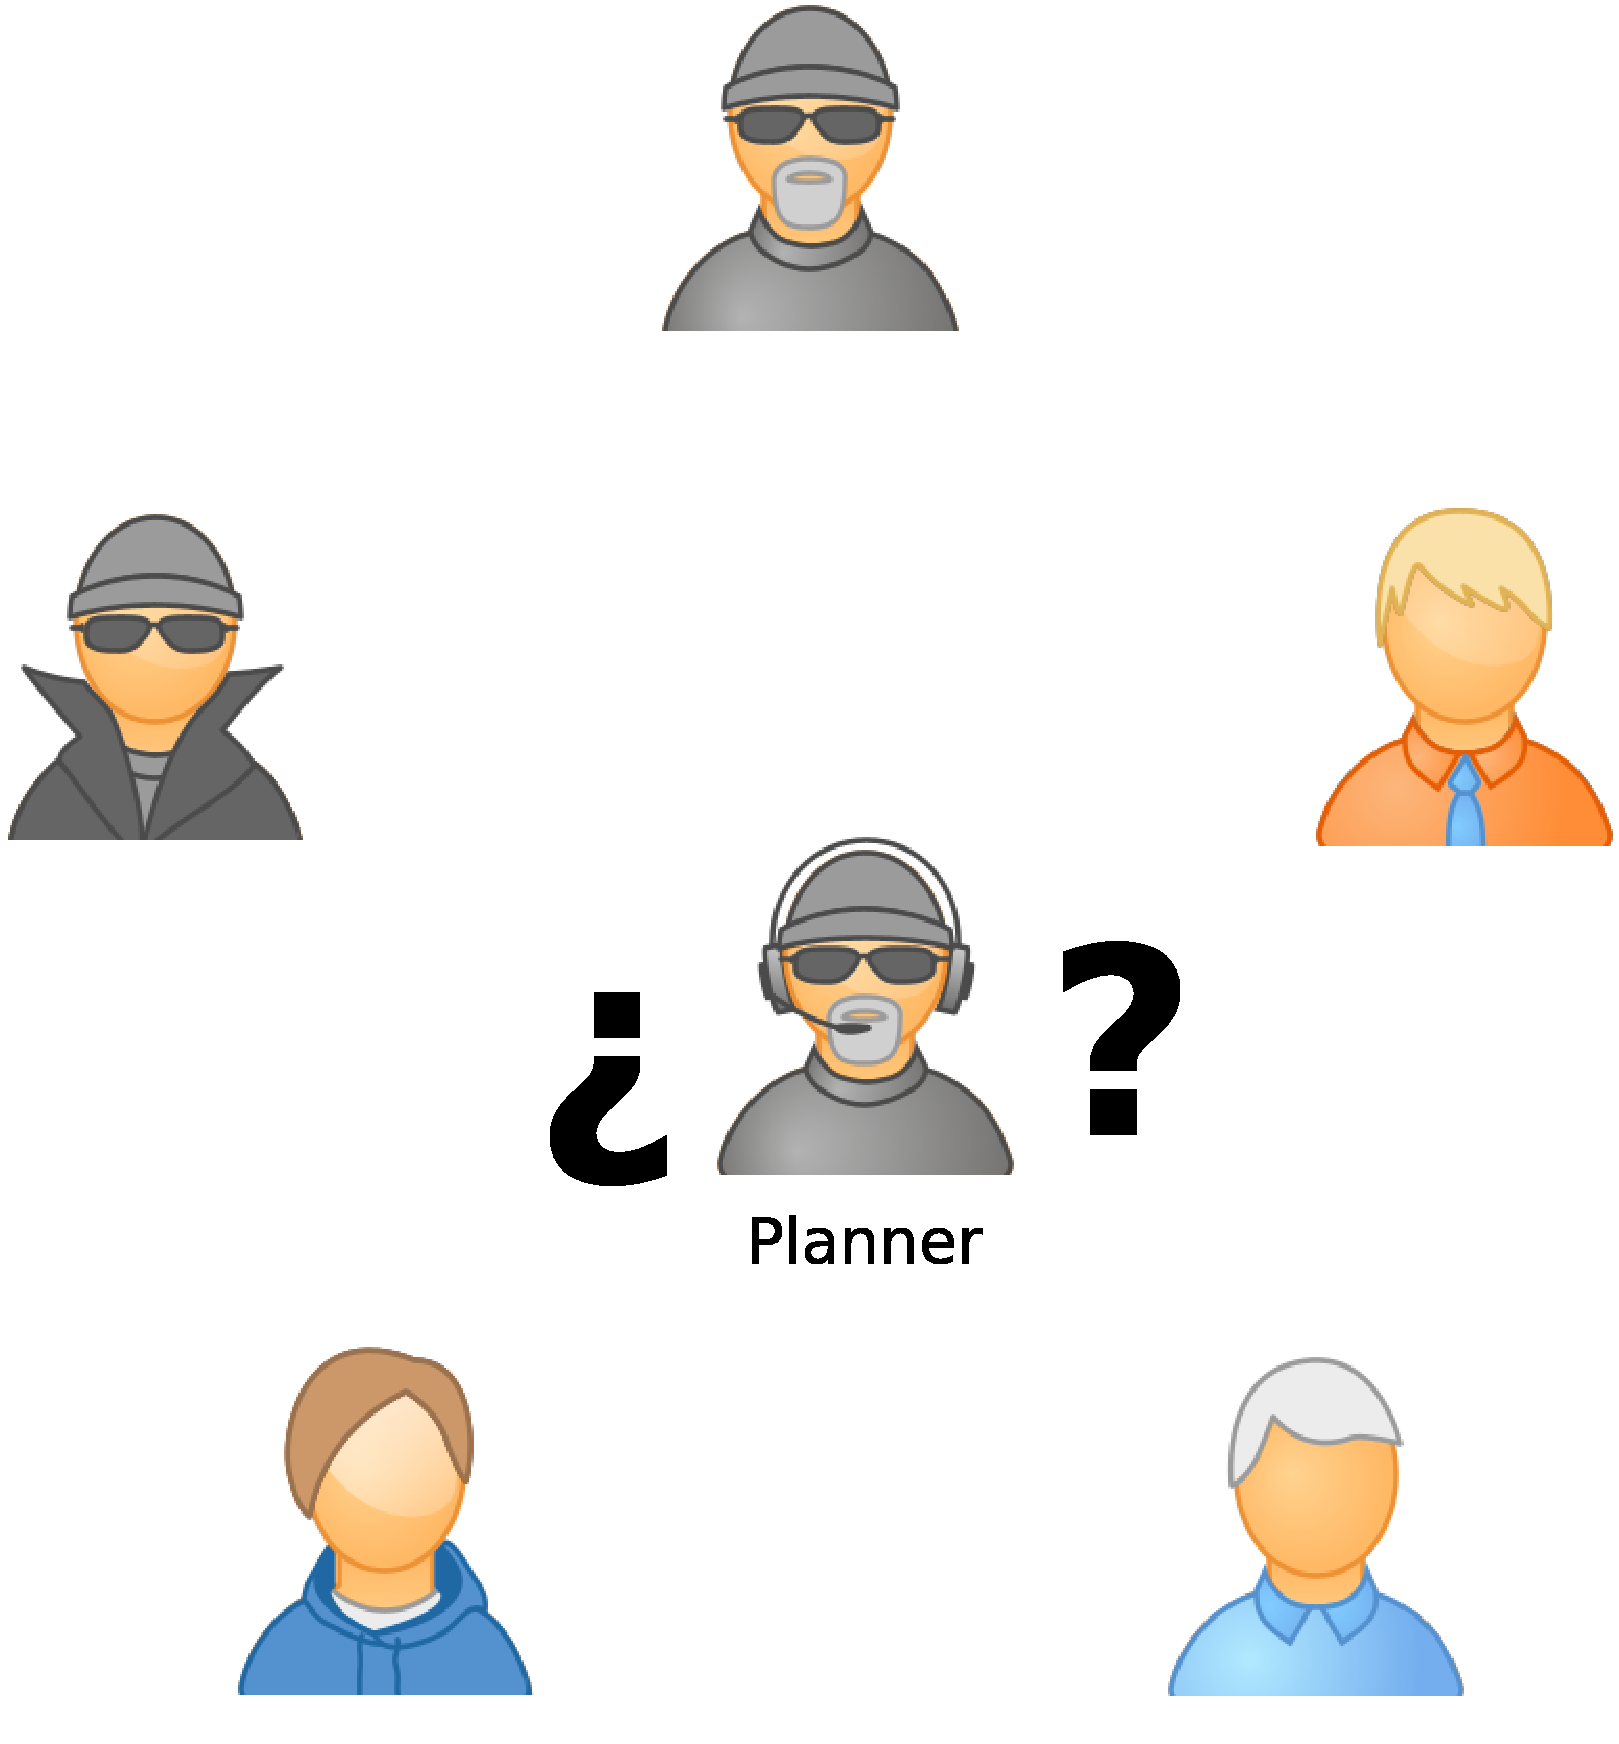
\includegraphics[width=0.7\textwidth]{images/planner-1.pdf}}%\caption{Figure ?}}
      \only<2->{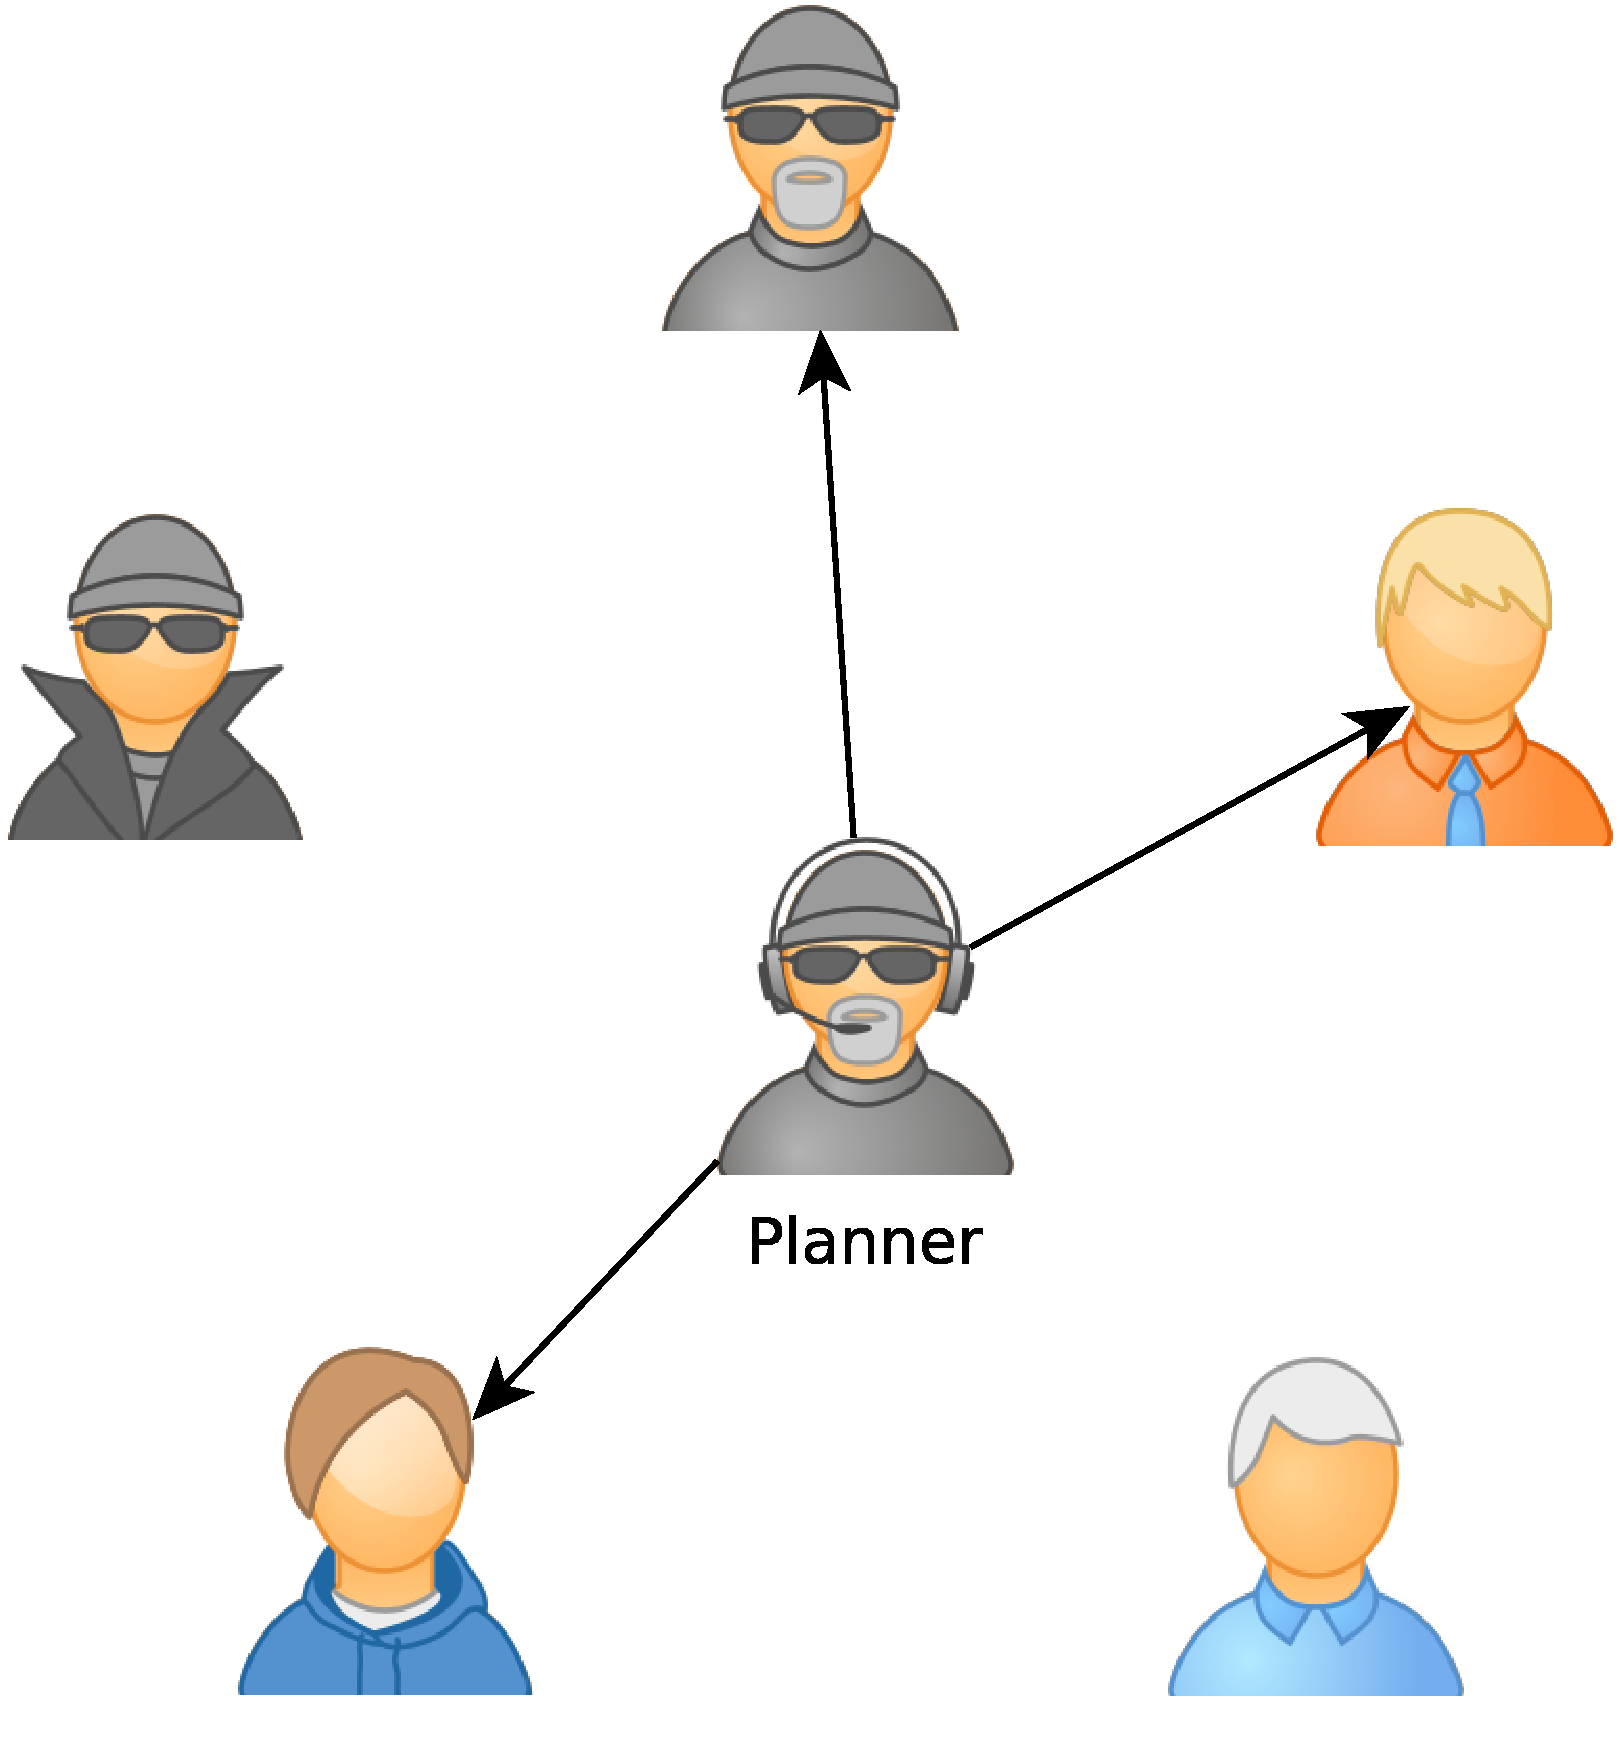
\includegraphics[width=0.7\textwidth]{images/planner-2.pdf}}%\caption{Figure ?}}
    \end{figure}
  \end{columns}
\end{frame}

\begin{frame}
\frametitle{Steiner tree rational association model (StRAM)}
  \begin{columns}
  \column{0.5\textwidth}
    \begin{enumerate}
      \item Criminal skills are represented by the criminal propensity $pcg$ and trustworthiness through social distance between individuals $d_{ij}$
      \item The social distance between two individuals is represented by a value between $0$ and $1$, where $1$ represents the maximum distance between them.
    \end{enumerate}
  \column{0.5\textwidth}
    \begin{figure}[ht]
      \centering
      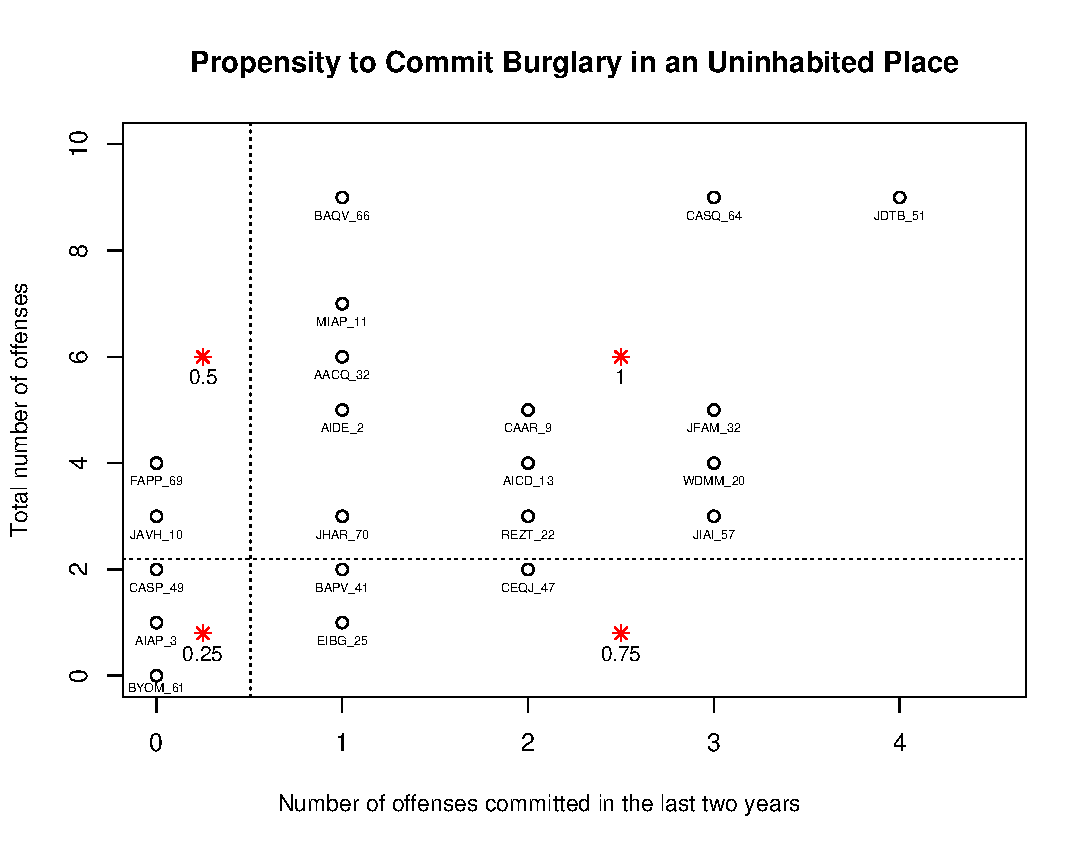
\includegraphics[width=\textwidth]{images/pcg_pdi.pdf}
      \caption{\footnotesize PCG values for network of 77 suspects}
    \end{figure}
  \end{columns}
\end{frame}

\begin{frame}
\frametitle{Steiner tree rational association model (StRAM)}
\begin{columns}
  \column{0.5\textwidth}
  \begin{block}{Objective function}
    \begin{itemize}
    \footnotesize
      \item Utility function of a crime planner
      \begin{equation*}
        \max U = \frac{\sum_{i \in N} pcg_i y_i}{pcg_{max} - pcg_s} - \frac{\sum_{(i,j) \in A} d_{ij} x_{ij}}{d_{max}}
      \end{equation*}
    \end{itemize}
  \end{block}
  \column{0.5\textwidth}
    \begin{block}{Decision variables}
    \footnotesize
      \vspace{1em}
      $y_{i} =
        \begin{cases}
          1 & \text{if $i \in N$ is in the criminal group}\\
          0 & \text{otherwise}
        \end{cases}$\\
      $x_{ij} =
        \begin{cases}
          1 & \text{if $(i,j) \in A$ is in the solution}\\
          0 & \text{otherwise}
        \end{cases}$\\
      $f_{ij} = \text{flow through the arc $(i,j) \in A$}$
    \end{block}
  \end{columns}
\end{frame}

\begin{frame}
\frametitle{Steiner tree rational association model (StRAM)}
\begin{block}{Constraints}
  \begin{scriptsize}
    \begin{columns}[t]
      \column{0.5\textwidth}
      \begin{itemize}
        \item Predecessor constraint:
        \begin{align}
          & \sum_{i \in N} x_{ij} = y_{j} & \forall j \in N \setminus \{s\} \\
          \intertext{\item Flow conservation:}
          & \sum_{i \in N} f_{ij} - \sum_{i \in N} f_{ji} = y_{j} & \forall j \in N \setminus \{s\} \\
          \intertext{\item Link of the variables:}
          & f_{ij} \leq (|N| - 1) x_{ij} & \forall (i,j) \in A
        \end{align}
      \end{itemize}
      \column{0.5\textwidth}
      \begin{itemize}
        \item Maximum criminal propensity:
        \begin{align}
          & \sum_{i \in N} pcg_i y_i \leq \varphi pcg_{max}\\
          \intertext{\item Variable’s domain:}
          & f_{ij} \geq 0 &\forall (i,j) \in A \\
          & x_{ij} \in \{0,1\} &\forall (i,j) \in A \\
          & y_{i} \in \{0,1\} &\forall i \in N
        \end{align}
      \end{itemize}
      \vfill
    \end{columns}
  \end{scriptsize}
\end{block}
\end{frame}

\section[Results]{Results}
\subsection[The Public Prosecutor’s Office of Chile Dataset]{The Public Prosecutor’s Office of Chile Dataset}

\begin{frame}
\frametitle{The Public Prosecutor’s Office of Chile Dataset}
\begin{columns}
  \column{0.5\textwidth}
  \begin{block}{The Public Prosecutor’s Office of Chile Dataset}
    \begin{itemize}
      \item The criminal network was provided by the criminal analysis unit of the Public Prosecutor’s Office of Chile.
      \item The database consists of 1,666 crimes and 77 suspects.
      \item The dataset contains a criminal group of 12 members.
    \end{itemize}
  \end{block}
  \column{0.5\textwidth}
    \begin{figure}[ht]
      \centering
      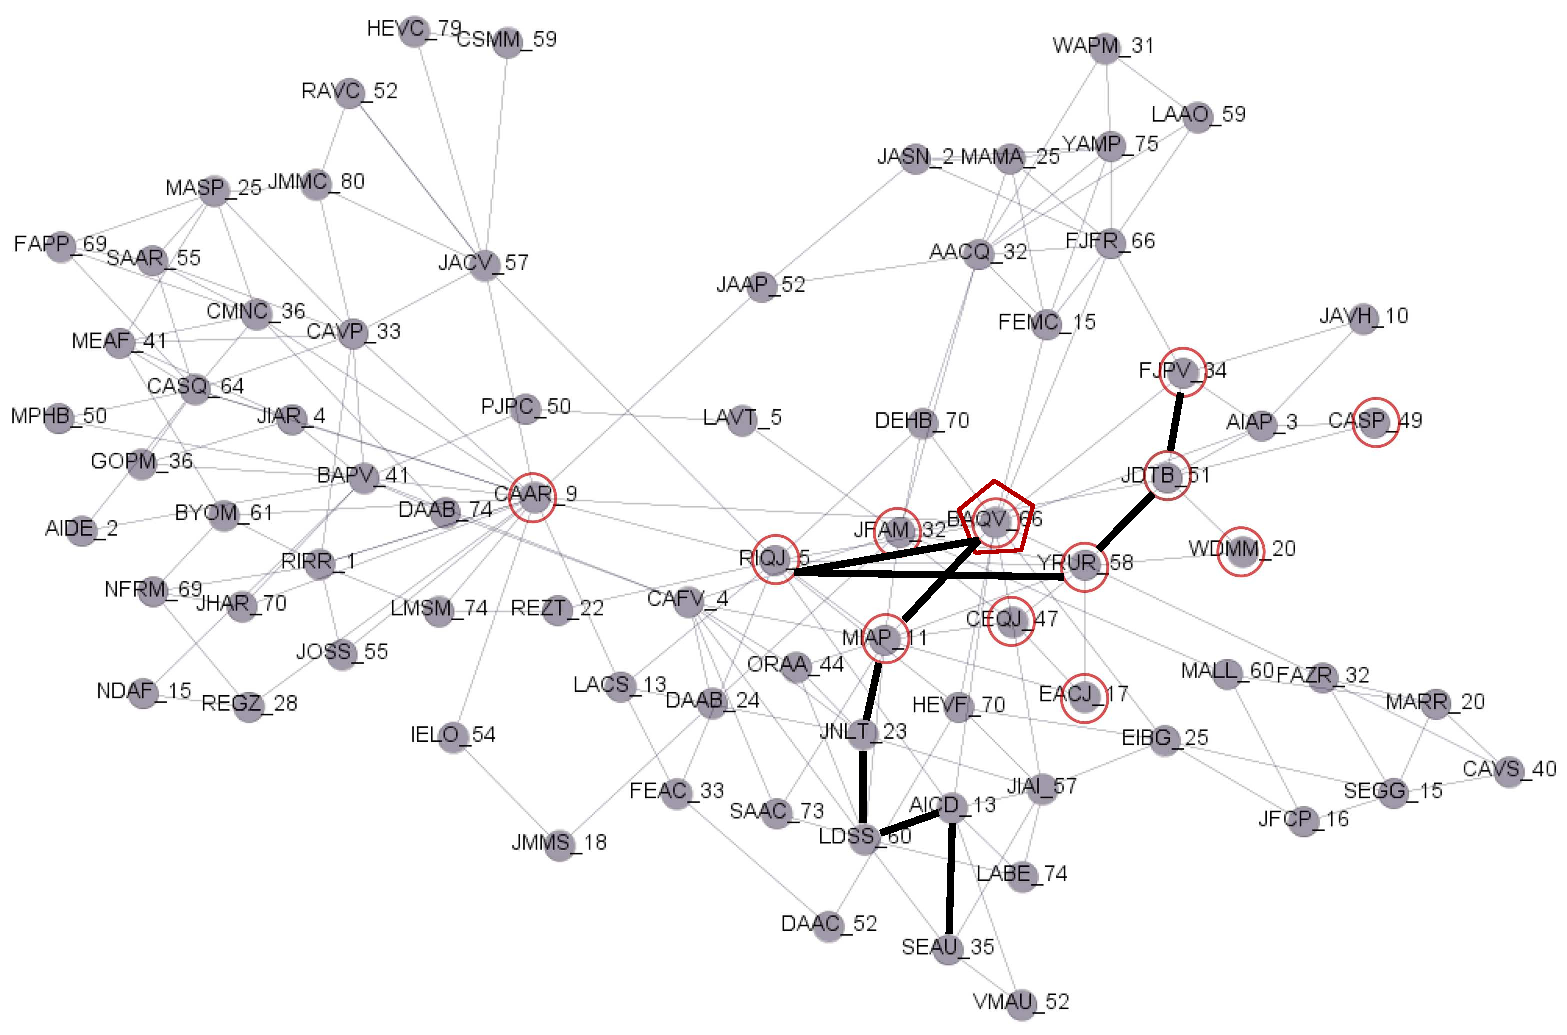
\includegraphics[width=\textwidth]{images/network.pdf}
      \caption{\footnotesize The network of 77 suspects.}
    \end{figure}
  \end{columns}
\end{frame}
\subsection[Test of the effectiveness of $StRAM$]{Test of the effectiveness of $StRAM$}
\begin{frame}
\frametitle{Test of the effectiveness of $StRAM$}
\begin{block}{Results}
  \footnotesize
  \begin{enumerate}
    \item The performance of this model is evaluated with the performance of the $LiRAM$\cite{Troncoso201} and $SPA$\cite{xu204} applied between pairs of suspicious individuals.
    \item $StRAM$ shows a slightly lower performance than $LiRAM$ for each value of $\varphi$.
    \item The confidence intervals intersect, therefore, there is no difference between the results of both models.
  \end{enumerate}
\end{block}
\begin{columns}
\column{0.45\textwidth}
  \begin{figure}[ht]
    \centering
    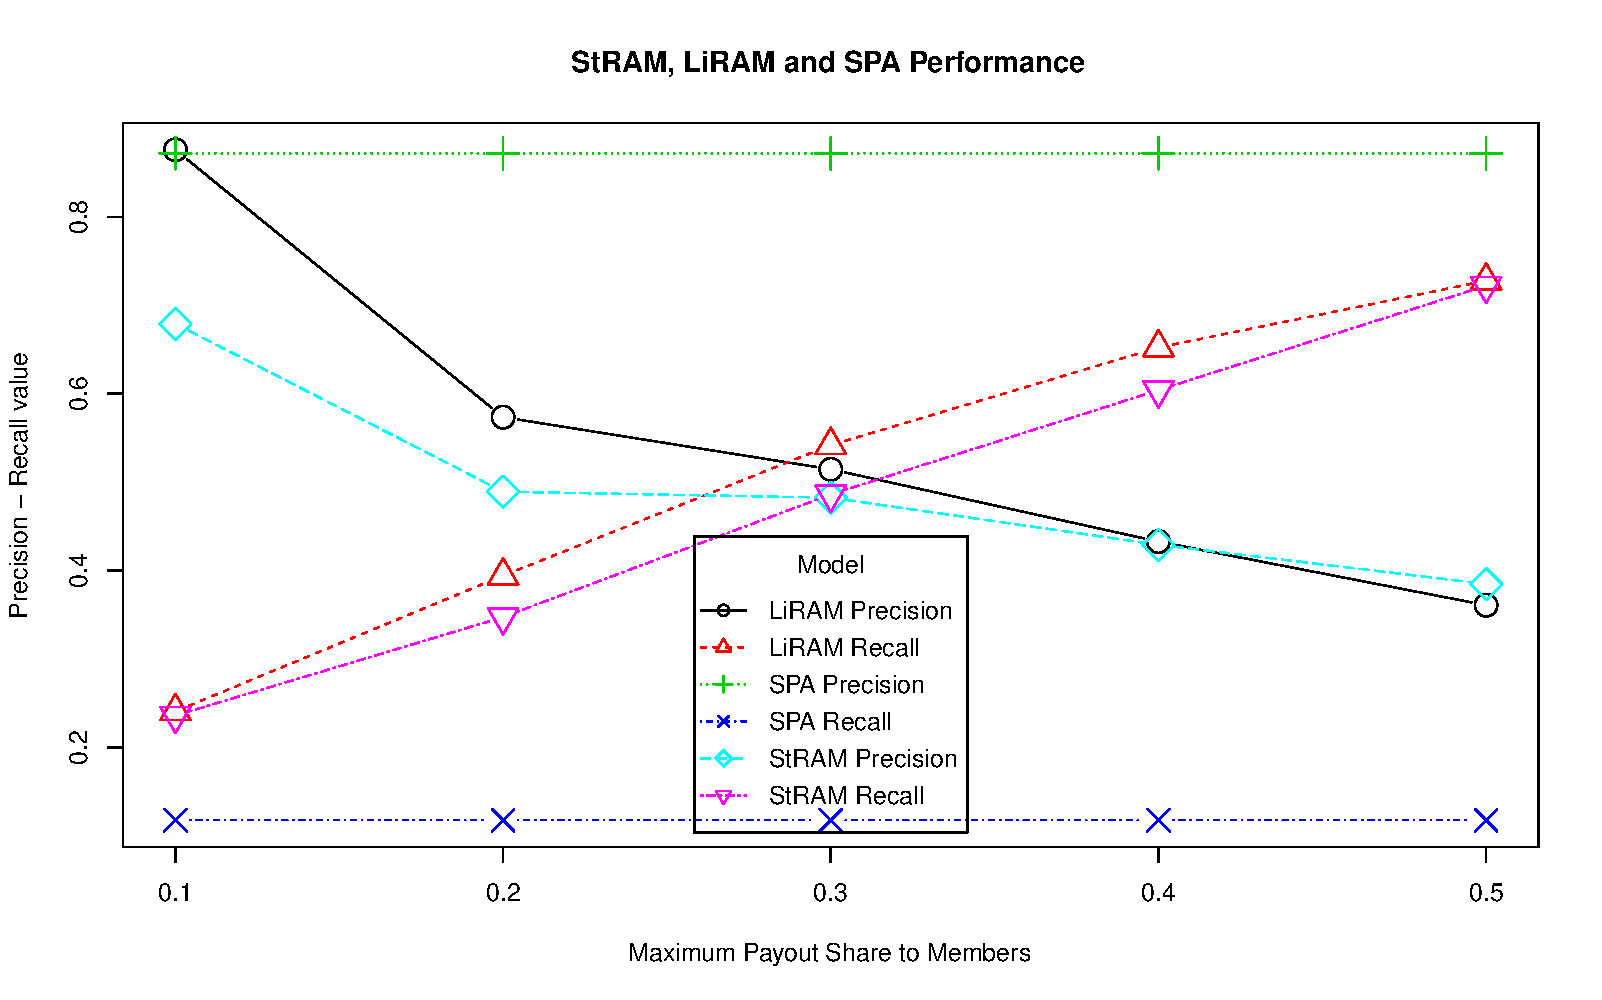
\includegraphics[width=0.8\textwidth]{images/comparation.pdf}
    \caption{\footnotesize Precision and Recall to StRAM, LiRAM and SPA.}
  \end{figure}
\column{0.55\textwidth}
  \begin{figure}[ht]
    \centering
    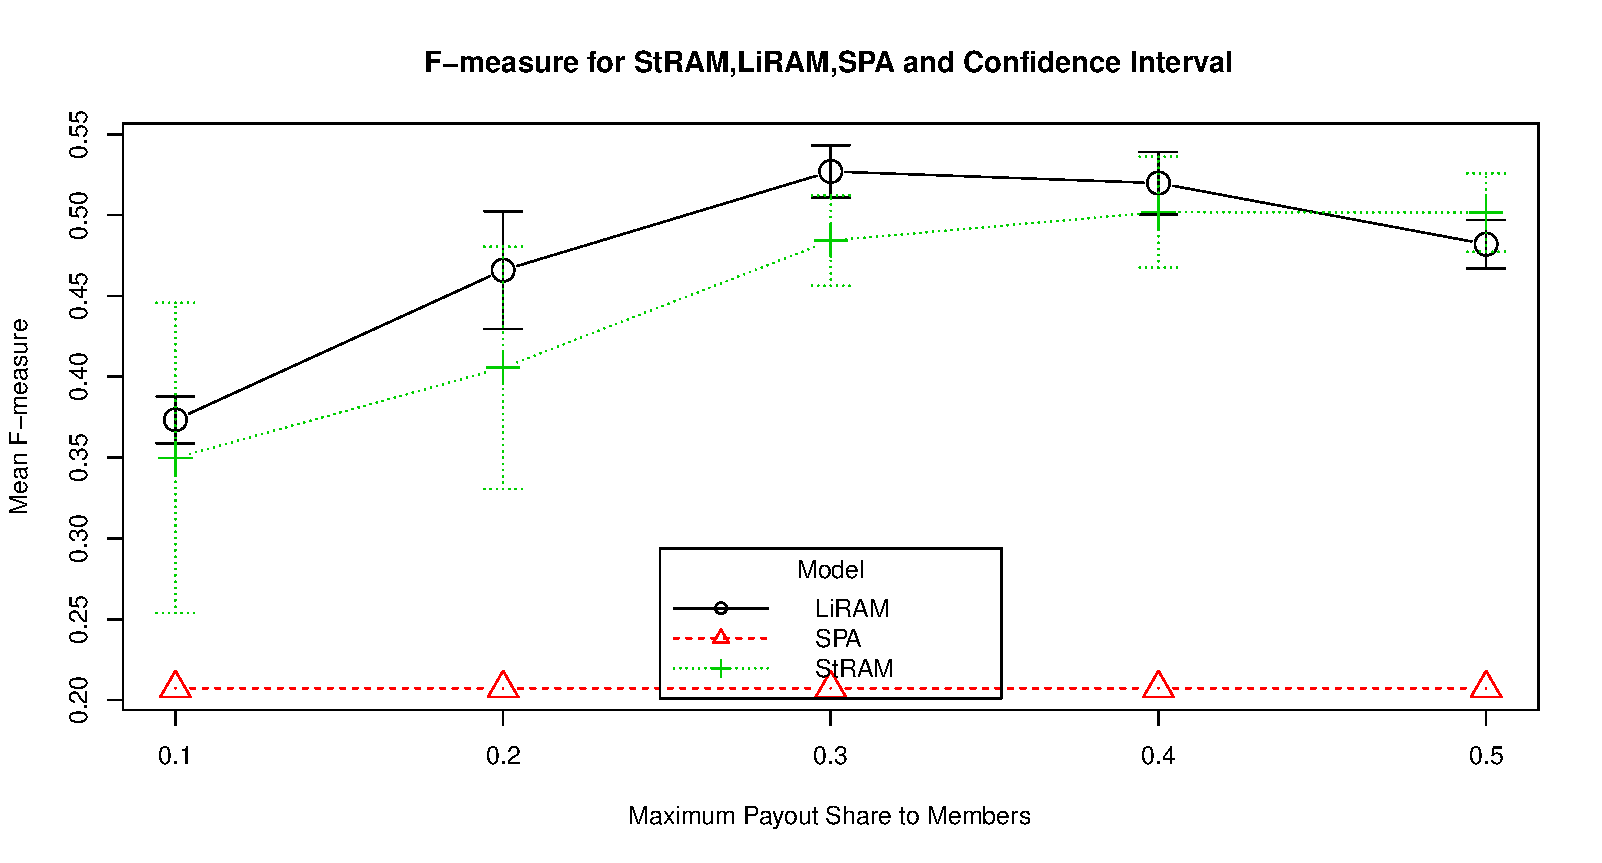
\includegraphics[width=0.8\textwidth]{images/confidence-interval.pdf}
    \caption{\footnotesize F-measure to StRAM, LiRAM and SPA}
  \end{figure}
\end{columns}
\end{frame}

\begin{frame}
\frametitle{Test of the effectiveness of $StRAM$}
\begin{block}{Results}
  \footnotesize
  \begin{enumerate}
    \item A statistical hypothesis test of mean difference between the models was applied.
    \item At a significance level of 0.05, the Shapiro-Wilk test indicates that the results are not normally distributed.
    \item Levene's test indicates that there is no homogeneity in the variance ($\alpha = 0.05$).
    \item The nonparametric Kruskal–Wallis test is applied. It is concluded that the results of both models are statistically similar ($\alpha = 0.05$).
  \end{enumerate}
\end{block}
\vfill
\begin{table}[ht]
  \scriptsize
  \centering
  \caption{\footnotesize Results to statistical tests for different values of $\varphi$.}
  \label{table:t1}
  \begin{tabular}{cccccc}
    \hline
                  \multicolumn{6}{c}{Results to Statistical Tests} \\ 
    \hline
                              & \multicolumn{5}{c}{Maximum Payout Share to Members P-value} \\ 
    \hline
    Test                      & $\varphi=0.1$   & $\varphi=0.2$ & $\varphi=0.3$ & $\varphi=0.4$  & $\varphi = 0.5$ \\
    Shapiro-Wilk (LiRAM data) & 0.0000000034111 & 0.0021649     & 0.0027877     & 0.0117392      & 0.2396275 \\
    Shapiro-Wilk (StRAM data) & 0.02501584      & 0.00374289    & 0.00201161    & 0.04011305     & 0.00056471 \\
    Levene                    & 0.00006102      & 0.1438        & 0.05163       & 0.03224        & 0.03611 \\
    Kruskal-Wallis            & 0.8504          & 0.4327        & 0.07577       & 0.6481         & 0.2407 \\ 
    \hline
  \end{tabular}
\end{table}

\end{frame}

\section[Conclusions and Future Work]{Conclusions and Future Work}
\begin{frame}
\frametitle{Conclusions}
  \begin{block}{Conclusions}
    \begin{enumerate}
      \item StRAM provides excellent results and even behaves comparably to existing approaches that start with two suspects.
      \item Many criminal investigations begin with a single suspect. Therefore, the proposed model opens new avenues for applied research in criminal investigation.
      \item Its application to a real-world case of crime analysis shows the potential StRAM has for crime investigation.
    \end{enumerate}
  \end{block}
  \begin{block}{Future Work}
    \begin{enumerate}
      \item It would also be interesting to apply StRAM without any confirmed cases and just using the propensity of members of potential suspects.
      \item We will sequentially apply StRAM and update the model parameters each time a new suspect is confirmed.
    \end{enumerate}
  \end{block}
\end{frame}

\begin{frame}[allowframebreaks]
  \frametitle{References}
  \footnotesize
  %\nocite{*}
  \bibliography{bibliography.bib}
\end{frame}

\begin{frame}
\frametitle{Acknowledgment}
\begin{columns}
\column{0.6\textwidth}
\begin{itemize}
\item FONDEF project ID20I10230ANID
\item The Initiation Research Project 2060204IF/I
\item Fondecyt Project 1181036
\item Project ING 2030 I+D 20-34.
\item Santiago based Complex Engineering Systems Institute (CONICYT PIA/BASALAFB180003).
\item The Criminal Analysis Unit of the Public Prosecutor's Office of Región del Biobío-Chile
\end{itemize}
\column{0.4\textwidth}
\centering

\includegraphics[width=0.5\textwidth]{logos/ubb}

\includegraphics[width=0.4\textwidth]{logos/uchile}
\vspace{0.5\baselineskip}


\includegraphics[width=0.45\textwidth]{logos/uandes}
\end{columns}
\end{frame}

\begin{frame}
  \titlepage
\end{frame}

\end{document}
